\section{Iterative Co-Segmentation and Joint Registration}
\label{sec:segmentation}
\subsubsection{Logic Outline}
\begin{table*}[!hbp]
	\begin{tabular}{p{0.15\textwidth}|p{0.25\textwidth}|p{0.25\textwidth}|p{0.25\textwidth}}
		\hline
		步骤 & 期望目标 & 目前算法实际达到的效果 & 主要差异\\
		\hline
		Region Grow 
		& 输入:一个由多个物体混在一起没有被label的区域(要求不能有一个物体部分被label而另一部分没有被label)
		输出:欠分割的结果—————将每一帧分为多个patch每一个patch由一个或多个物体组成 
		& 将每一帧中还没有被label的区域按照空间是否近邻分为多个patch 
		& 只要输入符合要求我认为在室内数据中是等价的
		\\
		\hline
		Clustering
		& 输入所有的patch, 输出每个patch所属类别,要求每一类所有的patch中最大的(所占点最多)物体都相同
		& 以patch最多的一帧的patch特征为初始用k-means来获取聚类中心,将每帧中特征空间中距离聚类中心最近的归为该类
		& 完全不等价,也没有满足需求\\
		\hline
		Joint Registration 
		& 输入同一类的patch,将它们按照类中patch共有的最大的物体配准到一起 
		& 输出一个模型与一组刚体变换,在存在noise和outlier的前提下,以高斯为先验最大化 后验概率————这些观察到的patch是由这个模型按照这组刚体变换生成的  
		& 并不等价,但是从结果来看我觉得是能够满足需求的 \\
		\hline
		Graph Cut
		& 将每一类的每个patch中除了主体物体之外的部分重新标记为没有被label的区域
		& 一个superpixel如果按照某个类的变换能够在每一帧都匹配得(如能量项中的取max就是为了表达需要在每一帧中都匹配得好才叫匹配得好)很好则label为这个物体,果都匹配得不好则重新被标记为没有label的区域(匹配得好与不好的门限的设置依然是不清晰的)
		& 因为噪声和形变的存在所以并不能够等价
	\end{tabular}
	\caption{Logic Outline v0.0} %表格的名称
	\label{tab:logic_outline00}
\end{table*}
\begin{table*}[!hbp]
	\begin{tabular}{p{0.15\textwidth}|p{0.75\textwidth}}
		\hline
		步骤 & 期望目标 \\
		\hline
		Region Grow&\tabincell{l}{
			输出:\\
			每一帧每个pixel有一个label值
			要求:\\
			1.在任意一帧中,属于同一个物体的pixel必须被赋予同一个label值。\\
			2.在任意一帧中,属于不同的物体的pixel也可以被赋予同一个label的值。\\(被赋予同一个label值的pixel被认为组成一个patch,\\则这项要求等价于一个patch可以是一个或多个物体的集合)\\
			3.在不同的帧之间,属于同一个物体的pixel不需要被赋予同一个label值。}\\
		\hline
		Clustering&\tabincell{l}{输出:\\
			每个patch赋予一个新的label的值,其中可以存在一个特殊的零label\\
			要求:\\
			1.在不同帧之间,同一个label(零label除外)的patch(称为同一个类的patch)必须包含\\同一个物体,且这个相同的物体在包含它的patch中占有的点的比例足够大(称为类内核心物体)\\
			2.允许原本多个patch被同时赋予零label}\\
		\hline
		Joint Registration&\tabincell{l}{
			输出:\\
			除了零label的patch以外,
			对于每一个patch得到一个刚体变换,对于每一类得到一个物体模型。\\
			要求:\\
			1.零label除外,每一类的patch按照所得到的刚体变换变换以后,\\这一类的类内核心物体将会在三维空间中对齐。}\\
		\hline
		Graph Cut&\tabincell{l}{输出:\\
			更新每个pixel的label,使得原本属于类内核心物体的pixel的label与原本类的label相同,\\
			而不属于类内核心物体的pixel的label被置为零label\\
			要求:\\
			1.允许部分属于类内核心物体的pixel被置为零label。\\
			2.不允许不属于类内核心物体的pixel保留原来该类的label。}\\
		\hline
		Region Grow&\tabincell{l}{输出:\\
			给每一个零label的pixel赋予一个非零的label值。\\
			要求:\\
			1.对于不属于上一步中类内核心物体的pixel要求符合第一次\\region grow的要求(属于新分出来的物体的pixel)。}\\
		\hline
		Clustering&\tabincell{l}{输出:\\
			每个patch赋予一个新的label的值,不存在零label
			要求:\\
			1.在不同帧之间,同一个label(零label除外)的patch(称为同一个类的patch)\\必须包含同一个物体,且这个相同的物体在包含它的\\patch中占有的点的比例足够大(称为类内核心物体)\\
			2.允许patch恢复为上一步聚类时的label值}\\
		\hline
	\end{tabular}
	\caption{Logic Outline v0.1} %表格的名称
	\label{tab:logic_outline01}
\end{table*}
\begin{table*}[!hbp]
	\begin{tabular}{p{0.15\textwidth}|p{0.75\textwidth}}
		\hline
		步骤 & 期望目标 \\
		\hline
		Region Grow&\tabincell{l}{
			输入:\\
			同一个场景不同时刻扫描的T个Point Cloud:$\{F_t\}$\\
			场景中总共包含没有被区分开的N个物体:$\{O_n\}$\\
			第n帧点云有$I(t)$个点,$p_{ti}$表示第N帧的第i个点\\
			输出:\\
			对于每一帧输出$J(t)$个Patch$\{P_{tj}\}$\\
			要求:\\
			1.Patch之间没有重叠。\\
			2.同一个物体不能分到两个不同的Patch中。\\
			3.不同的物体可以被分到同一个Patch中。\\
			}\\
		\hline
		Clustering&\tabincell{l}{
			输入:\\
			所有的Patch$\{P_{tj}\}$\\
			输出:\\
			将所有的Patch分配到M+1个类当中$\{C_m\}$\\
			其中$C_0$为无语义类,其余类为有语义类。
			要求:\\
			1.同一帧的两个Patch不能属于同一个有语义类。\\
			2.属于同一个有语义类的Patch必须包含同一个物体,并且这个物体在包含它的Patch中必须占有足够大的比例。(这个物体称为类内核心物体) 
			}\\
		\hline
		Joint Registration&\tabincell{l}{
			输入:\\
			已经被分配到个M+1类中的Patch\\
			设第m类有K(m)个Patch,则$P_{mk}$表示第M类的第k个Patch\\
			输出:\\
			除了$C_0$以及属于$C_0$的Patch之外,
			对于每一个$P_{mk}$得到一个刚体变换,\\
			对于每一类得到一个物体模型${M_m}$\\
			要求:\\
			1.除了属于$C_0$的Patch之外,每一类的Patch按照所得到的刚体变换变换以后,\\这一类的类内核心物体将会在三维空间中对齐。}\\
		\hline
		Graph Cut&\tabincell{l}{
			输入:(前一步的输出)\\
			输出:\\
			将不属于类内核心物体的点从该类的Patch中移除\\
			要求:\\
			1.允许部分属于类内核心物体的点被错误的移除。\\
			2.不允许没有被移除干净的点。}\\
		\hline
		Region Grow&\tabincell{l}{
			输入:\\
			前一步中被从Patch中移除的点。\\
			输出:\\
			从没有Patch归属的点中重新生成Patch\\
			要求:\\
			1.对于没有被错误移除的点要求在生成Patch时满足第一次region grow 的要求}\\
		\hline
		Clustering&\tabincell{l}{
			输入:\\
			上一步中新生成的Patch\\
			输出:\\
			将所有的新Patch分配到M个新的类当中$\{C_m\}$\\
			要求:\\
			1.同一帧的两个Patch不能属于同一个有语义类。\\
			2.属于同一个有语义类的Patch必须包含同一个物体,\\并且这个物体在包含它的Patch中必须占有足够大的比例。(这个物体称为类内核心物体)\\
			3.新生成的Patch如果不能被分配到一个有语义的类当中则\\将他合并回到之前的Patch中去。
			}\\
		\hline
	\end{tabular}
	\caption{Logic Outline v0.2} %表格的名称
	\label{tab:logic_outline02}
\end{table*}
\begin{table*}[!hbp]
	\begin{tabular}{p{0.15\textwidth}|p{0.75\textwidth}}
		\hline
		步骤 & 期望目标 \\
		\hline
		Region Grow&\tabincell{l}{
			输入:\\
			同一个场景不同时刻扫描的T个Point Cloud:$\{F_t\}$\\
			场景中总共包含没有被区分开的N个物体:$\{O_n\}$\\
			第n帧点云有$I(t)$个点,$p_{ti}$表示第N帧的第i个点\\
			输出:\\
			对于每一帧输出$J(t)$个Patch$\{P_{tj}\}$\\
			要求:\\
			1.Patch之间没有重叠。\\
			2.同一个物体不能分到两个不同的Patch中。\\
			3.不同的物体可以被分到同一个Patch中。\\
		}\\
		\hline
		Clustering&\tabincell{l}{
			输入:\\
			所有的Patch$\{P_{tj}\}$\\
			输出:\\
			将所有的Patch分配到M+1个类当中$\{C_m\}$\\
			其中$C_0$为无语义类,其余类为有语义类。
			要求:\\
			1.同一帧的两个Patch不能属于同一个有语义类。\\
			2.属于同一个有语义类的Patch必须包含同一个物体,并且这个物体在包含它的Patch中\\必须占有足够大的比例。(这个物体称为类内核心物体)\\
			3.应该考虑利用Joint Registration的反馈信息在不出错的前提下尽量多的将Patch分配到有语义的类当中。
		}\\
		\hline
		Joint Registration&\tabincell{l}{
			输入:\\
			已经被分配到个M+1类中的Patch\\
			设第m类有K(m)个Patch,则$P_{mk}$表示第M类的第k个Patch\\
			输出:\\
			除了$C_0$以及属于$C_0$的Patch之外,
			对于每一个$P_{mk}$得到一个刚体变换,\\
			对于每一类得到一个物体模型${M_m}$\\
			要求:\\
			1.除了属于$C_0$的Patch之外,每一类的Patch按照所得到的刚体变换变换以后,\\这一类的类内核心物体将会在三维空间中对齐。}\\
		\hline
		Graph Cut&\tabincell{l}{
			输入:(前一步的输出)\\
			输出:\\
			将不属于类内核心物体的点从该类的Patch中移除\\
			要求:\\
			1.允许部分属于类内核心物体的点被错误的移除。\\
			2.不允许没有被移除干净的点。}\\
		\hline
		Region Grow&\tabincell{l}{
			输入:\\
			前一步中被从Patch中移除的点。\\
			输出:\\
			从没有Patch归属的点中重新生成Patch\\
			要求:\\
			1.对于没有被错误移除的点要求在生成Patch时满足第一次region grow 的要求}\\
		\hline
		Clustering&\tabincell{l}{
			输入:\\
			上一步Region Grow中新生成的Patch\\
			输出:\\
			将所有的新Patch分配到M+N个类当中$\{C_m\}$\\
			要求:\\
			1.首先尝试将新Patch分配到原有的类当中,再利用其中剩下聚类产生新的类。\\
			2.同一帧的两个Patch不能属于同一个有语义类。\\
			3.属于同一个有语义类的Patch必须包含同一个物体,\\并且这个物体在包含它的Patch中必须占有足够大的比例。(这个物体称为类内核心物体)\\
			4.新生成的Patch如果不能被分配到一个有语义的类当中则\\将他合并回到之前的Patch中去。
		}\\
		\hline
	\end{tabular}
	\caption{Logic Outline v0.3} %表格的名称
	\label{tab:logic_outline03}
\end{table*}
如Figure~\ref{fig:iterative-segmentation-registration}所示展示了迭代分割与配准的系统流程。
\begin{figure*}
	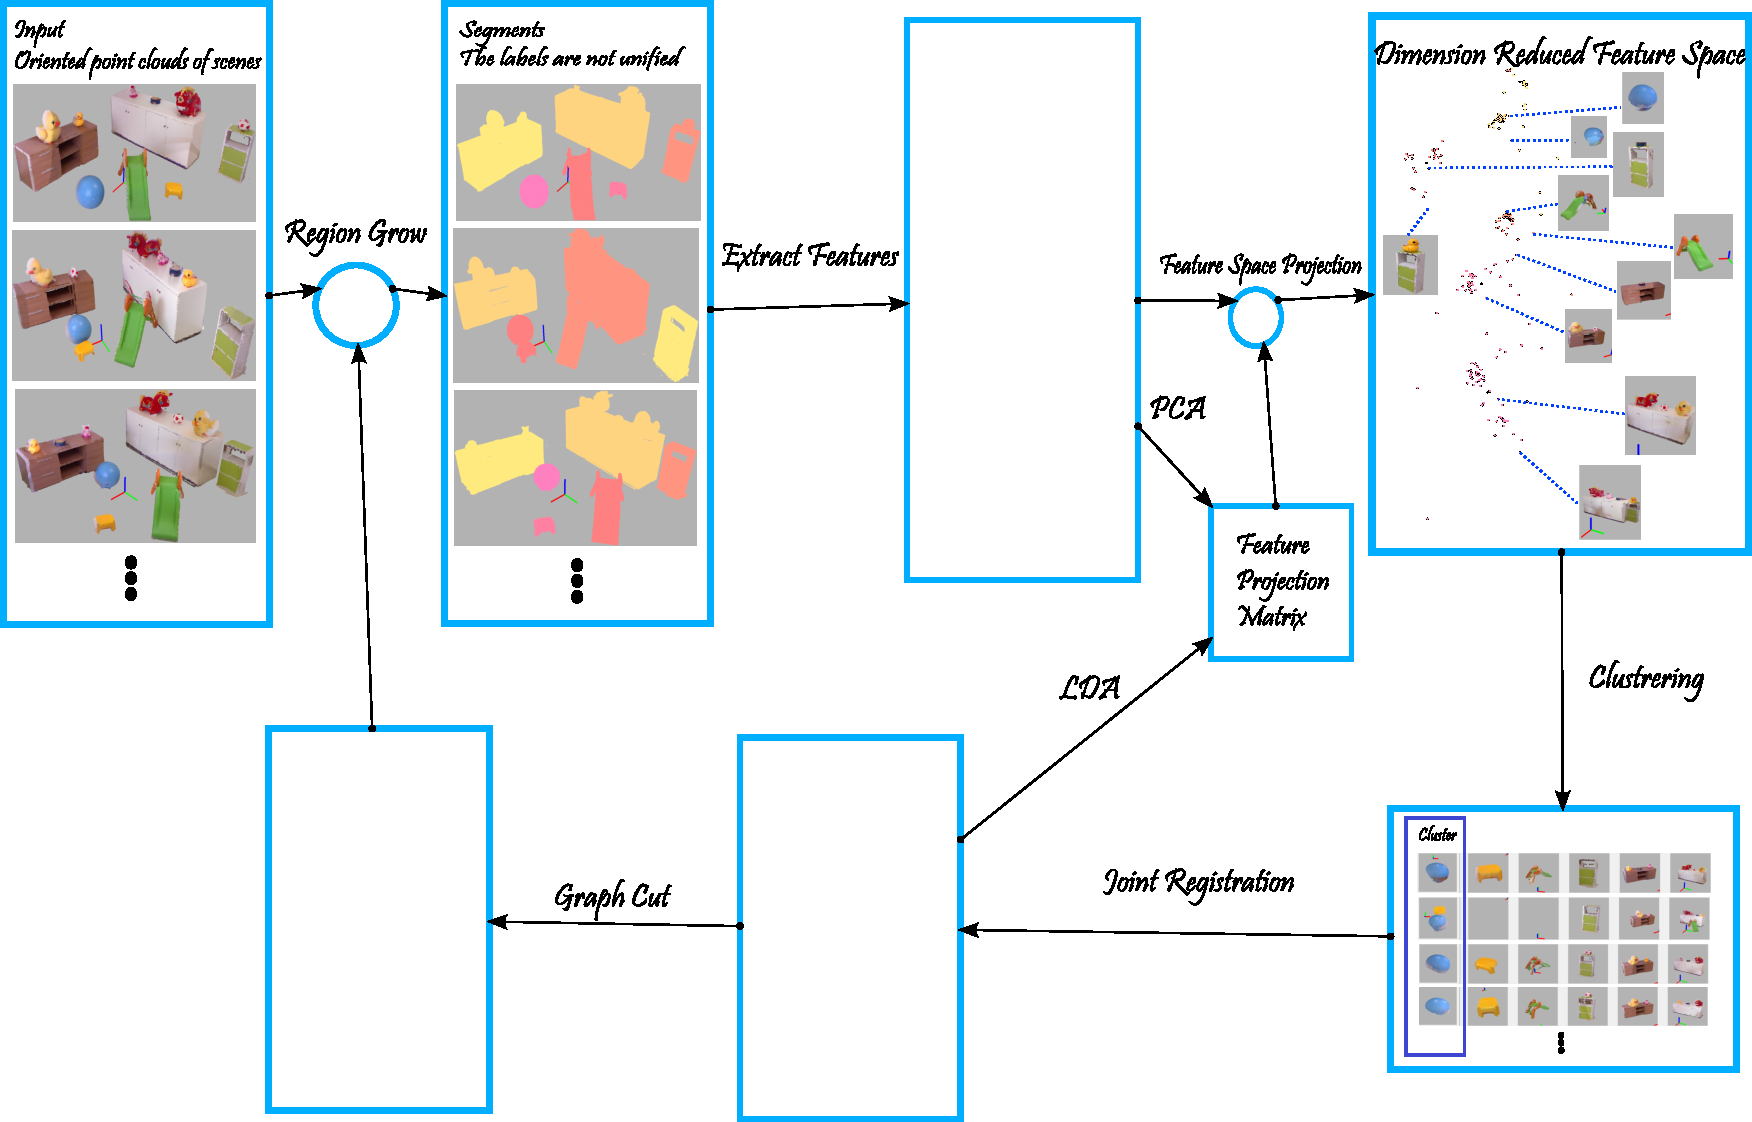
\includegraphics[width=1.0\textwidth]{figures/hsy/overview}
	\caption{Iterative co-segmentation and joint registration.}
	\label{fig:iterative-segmentation-registration}
\end{figure*}
\subsection{Region Grow}
区域生长的操作是对每一帧独立进行的。\\
输入是每一帧的点云以及每一帧所对应的label。\\
输出是更新之后的label。 \\
所谓label就是一个整数的数组它赋予点云中每一个点一个$id$,用来指示它所属的分割区域。我的实现中默认$id=0$的区域是未知区域(在图示中对应黑色区域)。在最开始时label的初始值是全为0。\\
区域生长操作是针对每一帧中的未知区域进行的,所使用的准则是如果两个区域之间有点互相在以R(默认$R=0.02$)为半径的邻域中就将这两个区域合并为同一个区域。\\
选择这样的准则基于的假设是相距较远且不连续的两组点云不太可能属于同一物体。\\
我们认为这样的准则会自然得到欠分割(under-segment)的分割结果。以便于后续能够进行配准(registration)操作\\
Figure~\ref{fig:object-iterations} 显示了第一次与第二次区域生长的过程。
\subsection{Object Clustering ( Unify Label )}
这一步操作是将每一帧的不同分割区域的patch无监督的聚成多个类以便于后续对每一类进行配准(registration)。
这一步输入是所有的点云以及它们对应的label,输出仍然是更新之后的label。
先依照前一步的label将点云分成多个patch,对所有的patch提取特征,然后依据投影矩阵将特征降维,然后再在低维空间中根据聚类中心为每一个patch重新分配id并更新每一帧的label。\\
关于使用了哪些特征?\\
如何得到投影矩阵?\\
如何确定聚类中心?\\
以下分别进行说明:
\subsubsection{Features}
Table~\ref{tab:features}列举了所有使用的特征以及对应的维数。
其中后三种feature实际上是以bounding box为参考提取的关于物体形状的特征。
\begin{table}[!hbp]
\begin{tabular}{p{0.73\columnwidth}|{p{0.1\columnwidth}}}
\hline
Feature & Dimension & \\
\hline
~\\
RGB Color Histogram & 125\\~\\
Size of Bounding Box & 3\\~\\
Percentage of Points Closest to Front-Back Left-Right Up-Down of its Bounding Box & 3\\~\\
Mean Distances to its Bounding Box ( Seperately Accounted for Front-Back Left-Right Up-Down  ) & 3 \\~\\
Standard Deviation of Distances to its Bounding Box ( Seperately Accounted for Front-Back Left-Right Up-Down  ) & 3
\end{tabular}
\caption{Patch Features} %表格的名称
\label{tab:features}
\end{table}
\subsubsection{Projection Matrix}
为什么降维,以及降维维数的选择:\\
1.将特征向量进行线性投影相当于为不同的特征赋予不同的权重来衡量。\\
2.之所以降维是为了后续能够进行k-means更新聚类中心。 k-means相当于一个简化的混合高斯的估计过程, 而要有效估计一个一维的高斯模型就按只需要五个样本(一般估计一个线性模型都至少要五个样本)来算,二维的要达到同样的采样密度需要25个样本,三维则需要至少125个样本。而我们的每组数据实际只有不到一百帧每个物体都没有125个这么多的样本。因此我认为降维到两维是合理的选择,同时这也方便对特征空间进行visualize。\\
降维的方法:\\
初始时投影矩阵是对所有patch的特征做PCA来生成的.
后续则根据配准的结果进行LDA来获得,使用LDA相当于学习一组新的特征权重来重新衡量。LDA获得的新的投影矩阵应会使得特征在新的子空间内的类内方差变小类间方差变大。类与类之间的可区分度更好。
具体的做法在章节~\ref{subsec:registration}中的对应小节中还会仔细说明。
\subsubsection{Cluster Centers}
聚类是在投影后的特征子空间内进行的,初始时候聚类中心是将patch最多的一帧的patch所对应的特征点作为聚类中心,然后进行k-means更新聚类中心。
再进行registration之后还会根据registration的结果再更新聚类中心。具体细节在具体的做法在章节~\ref{subsec:registration}中的对应小节中还会仔细说明。
\subsubsection{Cluster Assignment}
算法~\ref{alg:assignment}说明了根据聚类中心在特征子空间中为一帧中的每个patch指定类别的算法过程,目的在于要保证每一帧中最多有一个patch被指定到某个类别。
\begin{algorithm}[htb]
\caption{Assign Patch to Cluster}
\label{alg:assignment}
\textbf{Input:}~~\\
$\{P_i\}$:Patch Features of One Frame~~\\
$\{C_j\}$:Cluster Centers~~\\
\textbf{Output:}~~\\
$\{Id_i\}$:Identity for Each Patch in this Frame
\begin{enumerate}
\item Calculate Distance Matrix $D_{ij}:=eucl\_dist(P_i,C_j)$
\item Set Column Index $CIndex: = 1:J$
\item Set Row Index $RIndex: = 1:I$\\
\textbf{while} $D$ is not empty \textbf{do}
\item Find~~$(i,j)=min(D)$
\item Set $Id_{RIndex(i)}:=CIndex(j)$
\item Remove Row $i$ and Column $j$ from $D$
\item Remove Element $i$ from $RIndex$
\item Remove Element $j$ from $CIndex$\\
\textbf{end while}
\end{enumerate}
\end{algorithm}
\subsection{Joint Registration}
\label{subsec:registration}
联合配准的步骤参考\cite{Evangelidis-ECCV-2014}的算法把之前步骤中被分为同一类的patch进行配准,对于整个系统而言这一步主要起到以下几方面的作用:\\
1.为之前的聚类结果提供反馈。(更新特征投影矩阵和聚类中心)\\
2.建立起帧与帧之间的对应关系。为后续的联合分割能量项的生成提供桥梁。\\
3.在最后的迭代中配准生成的物体模型将作为结果输出。\\
\subsubsection{Remove Unreliable Cluster Center By Registration Result}
Figure~\ref{fig:bedroom_O}中展示了若干个联合配准(joint registration)之后将各个patch对齐摆放后的图片。我们以配准的结果模型为参考计算各个patch与object模型match的程度,Figure~\ref{fig:bedroom_O}中的分数显示的是match的得分的分布情况包括最小值(min),最大值(max),均值(mean),中值(med),方差(var),标准差(stddev).我现在使用均值(>0)与标准差(<0.1)上设置阈值来判断是否为有效地聚类中心。(Figure~\ref{fig:bedroom_O}中\ref{fig:subfig:e}所示的床头柜实际混入了不少其它patch)
其中匹配程度的得分计算如下:
$$Score=\frac{1}{N}\sum_{(i,j)\in M }\frac{\vec{n_i}\vec{n_j}}{1+\alpha||p_i-p_j||} $$
其中$N$表示object model点的数量 M是以object model搜索patch中最近点所生成的点对的集合,$\vec{n}$表示点法向量,$p$表示点的空间位置。$\alpha$是一个参数。
对于不满足阈值的类就去除掉,这是为了避免错误的配准对后续步骤造成破坏,对于不确定的聚类留到下一次迭代再考虑。
为什么不是越匹配越好?而还要对匹配的得分的标准差做约束:
我们实际上是将以某个物体为核心的一大块区域放在一起做配准,匹配程度低很可能只是说明除了核心物体外混入的物体其它物体较多,而并不能说明这个聚类不是我们想要的。例如Figure~\ref{fig:subfig:g}比Figure~\ref{fig:subfig:e}匹配得分的均值要小就是因为以桌子为主体的patch中混入的其它物体较多。
\begin{figure*}
	\centering
	\subfigure[
	Invalid Object\\
	min:0.0494,max:0.6272\\
	mean:0.4763,med:0.5639\\
	var:0.0306,stddev:0.1749
	]{\label{fig:subfig:a}
	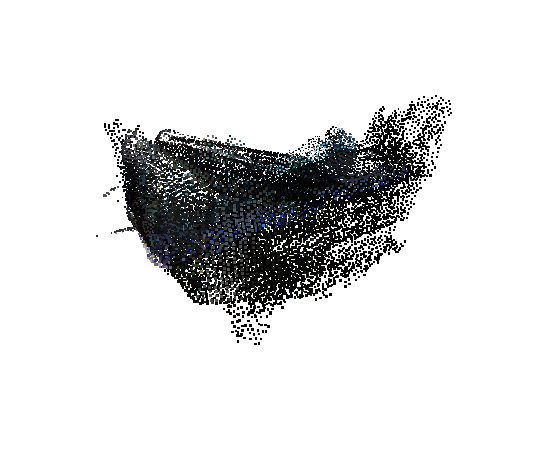
\includegraphics[width=0.2\textwidth]{figures/hsy/bedroom_O00.png}}
	\subfigure[
	Monitor\\
	min:0.7006,max:0.8442\\
	mean:0.7937,med:0.8033\\
	var:0.0012,stddev:0.0360
	]{
		\label{fig:subfig:b}
		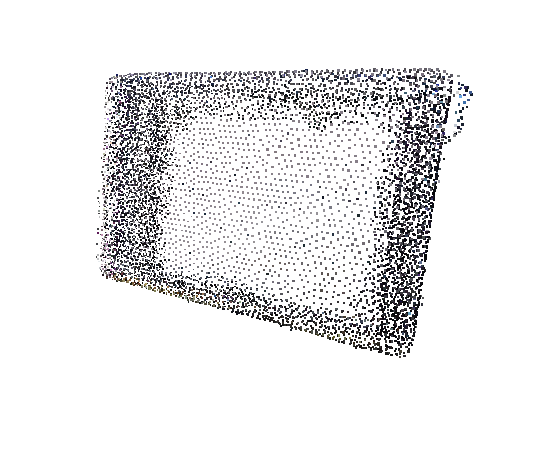
\includegraphics[width=0.2\textwidth]{figures/hsy/bedroom_O01.png}
	}
	\subfigure[
	Vacuum Sweeper\\
	min:0.5714,max:0.7993\\
	mean:0.7278,med:0.7503\\
	var:0.0031,stddev:0.0555
	]{
		\label{fig:subfig:c}
		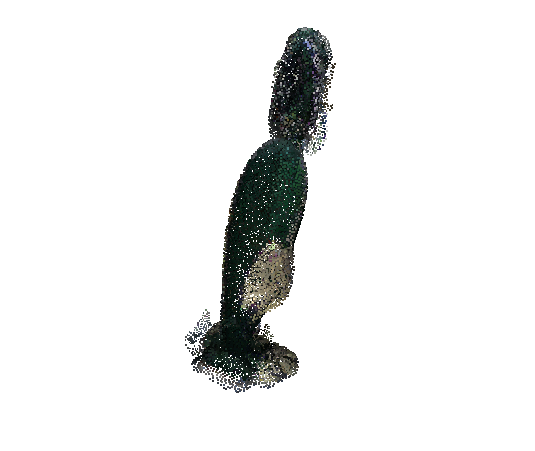
\includegraphics[width=0.2\textwidth]{figures/hsy/bedroom_O02.png}
	}
	\subfigure[
	Invalid Object\\
	min:-0.1001,max:0.5751\\
	mean:0.1733,med:0.1071\\
	var:0.0384,stddev:0.1961
	]{
		\label{fig:subfig:d}
		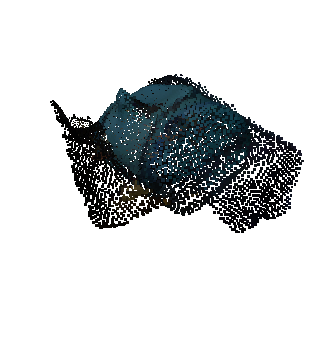
\includegraphics[width=0.2\textwidth]{figures/hsy/bedroom_O03.png}
	}
	\subfigure[
	Bed Stand(Mainly)\\
	min:0.2278,max:0.6439\\
	mean:0.5249,med:0.5707\\
	var:0.0134,stddev:0.1159
	]{
		\label{fig:subfig:e}
		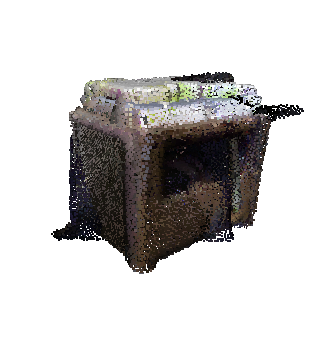
\includegraphics[width=0.2\textwidth]{figures/hsy/bedroom_O04.png}
	}
	\subfigure[
	Chair\\
	min:0.5774,max:0.7348\\
	mean:0.6731,med:0.6736\\
	var:0.0014,stddev:0.0380
	]{
		\label{fig:subfig:f}
		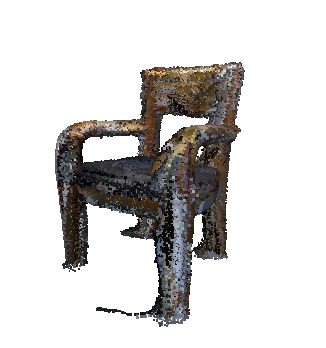
\includegraphics[width=0.2\textwidth]{figures/hsy/bedroom_O05.png}
	}
	\subfigure[
	Desk\\
	min:0.2860,max:0.4823\\
	mean:0.4130,med:0.4253\\
	var:0.0020,stddev:0.0449
	]{
		\label{fig:subfig:g}
		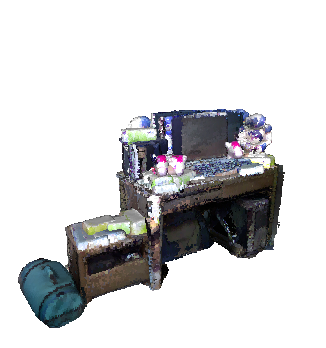
\includegraphics[width=0.2\textwidth]{figures/hsy/bedroom_O06.png}
	}
	\subfigure[
	Bed\\
	min:0.5031,max:0.6298\\
	mean:0.5787,med:0.5699\\
	var:0.0012,stddev:0.0350
	]{
		\label{fig:subfig:h}
		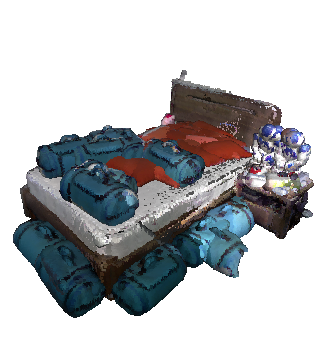
\includegraphics[width=0.2\textwidth]{figures/hsy/bedroom_O07.png}
	}
	\caption{Registered Object Models and Scores}
	\label{fig:bedroom_O}
\end{figure*}
\subsubsection{Update Project Matrix By Registration Result}
我选择使用LDA的方法来更新特征投影的矩阵主要出于以下几点考虑:
1.与初始的聚类方法能够较好的衔接(实现上只需要更新一个矩阵就好了)。\\
2.LDA相当于对不同维的特征赋予不同的权重使得类内方差尽量小而类间方差尽量大,从而在特征子空间中增加不同类别之间的可区分度。
Figure~\ref{fig:bedroom_pca_lda} 显示了PCA投影产生的特征子空间与LDA投影产生的特征子空间的对比。
\begin{figure*}
	\centering
	\includegraphics[width=2\columnwidth]{figures/hsy/bedroom_feature_compare}
	\caption{Feature Space Different Projection Matrix}
	\label{fig:bedroom_pca_lda}
\end{figure*}
\subsection{Global Consistent Graph Cut}
这一步主要利用之前配准所获得object model以及对应的刚体变换为中介来进行重新分割具体的能量项的设计如下:\\
重新分割操作是在每一帧上单独进行,但是其中data项的计算是通过与其它帧的比较来计算获得:\\
smooth term:\\
$$E(p_i,p_j,L_i,L_j)=\left\{
\begin{aligned}
& \sum_{(i,j)\in M }\frac{|\vec{n_i}\vec{n_j}|}{(1+\alpha||p_i-p_j||)(1+\beta||c_i-c_j||)}~&~L_i \neq L_j\\
& 0~&~otherwise
\end{aligned}
\right.
$$
其中:$\vec{n}$表示superpixel的法向量$p$表示空间位置,$c$表示RGB色彩。$\alpha$ 和 $\beta$ 是常数(目前实际取值就是1)\\
data term:\\
$$ E(p_i,L_i) =\left\{
\begin{aligned}
& C~&~L_i=0\\
& ||p_i-p_k|| + \max_{N}(\frac{||T_{nk}(p_i)-p_{nk}||}{T_{nk}(\vec{n_i})\vec{n_{nk}}})~&~L_i=1...K
\end{aligned}
\right $$
其中C是一个很大的常数,相当于一个门限,倘若label成任何一个物体都误差都超过C的时候希望被label为0。
其中$p_k$是通过$p_i$在当前帧中对应于第k个object的patch中找到的最近点。$T_{nk}(p_i)$是根据第k个object将点的空间位置$p_i$变换到第n帧相应的$T_{nk}(\vec{n_i})$是将法向量进行变换。$p_{nk}$是与$T_{nk}(p_i)$最近的点。$||p_i-p_k||$这一项的加入是为了应对存在多个不运动,或运动始终相同的物体时鼓励将当前点label为最近的点所属的物体。
\label{subsec:graphcut}
\begin{figure*}
\centering
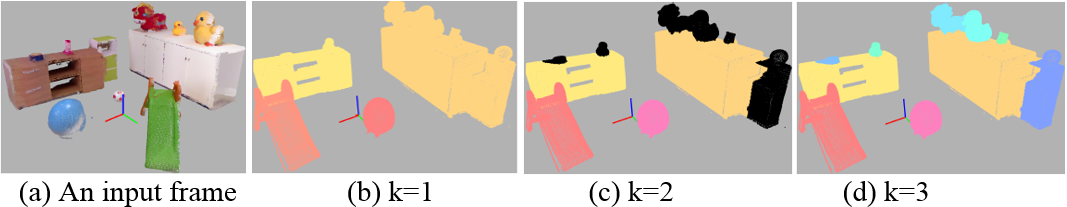
\includegraphics[width=2\columnwidth]{figures/object-iterations.png}
\caption{ The segmentation of each frame is progressively refined based on registered object models. From left to right: an input point cloud (a), segmentation updates at three iterations. \xj{show corresponding object model at each iteration.}}
\label{fig:object-iterations}
\end{figure*}
